\subsection{Reward and Value function}
% \todo{Ilk paragraf} 

As defined in the Markov Chain section, rewards and value functions are the essence of value iteration algorithms. In this section, we will describe the objective of the RL problem formally. As we mentioned in previous chapters, we want to increase the sum of rewards we achieve at the terminal state. If we define the reward at the final state \(T\) as \(R_T\) and the reward at the initial state \(t\) is \(R_t\), the returns we receive is the sum of rewards in every state.

\begin{equation}
    G_t = R_{t+1} + R_{t+2} + R_{t+3} + ... + R_T    
\end{equation}


\(G_t\) is the notation of expected return. We will mostly use the discounted version of the expected return calculation. We introduce a discount factor \(\gamma\) to value the rewards that the agent receives now, compare to the rewards in the future. 
\begin{equation}
    G_t = R_{t+1} + \gamma^1*R_{t+2} + \gamma^2*R_{t+3} + ... + \gamma^T-1*R_T = \sum\limits_{k=0}\gamma^kR_{t+k+1}
\end{equation}

For instance, if a rational human offered to choose between one million Euros now, versus one million Euros in 50 years, would usually choose one million Euros now. Therefore, our agent also weighs the rewards it receives now, over 50 steps from the current state.  In the meantime, we do not want the agent to undervalue the importance of reaching the terminal state through the highest reward sequence.  Given the below example (\ref{fig: nonoptimal}), if we introduce a discount factor of 0, the agent will always try to maximize the immediate reward and take a sequence of s1-a2-s3-a4-s4 and end up with a non-optimal greedy algorithm with \(G_t = 20 \). But with a discount factor, in this example everything between \(0< \gamma < 1\) works, would find the optimal sequence  s1-a1-s2-a3-s4 with \(G_t = 25\).

\begin{figure}[!htbp]
    \centering
    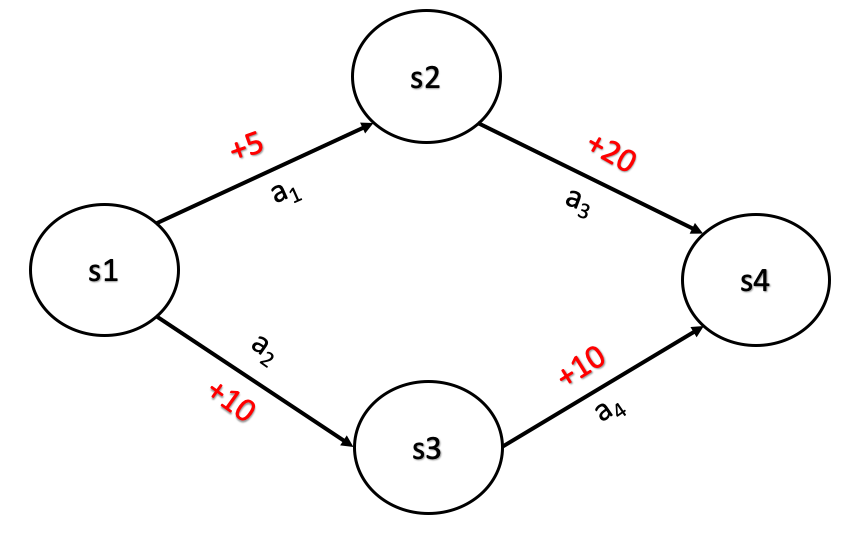
\includegraphics[width=0.6\textwidth]{figures/nonoptimal}
    \caption{Zero discount factor leads to non-optimal solution with s1-a2-s3-a4-s4. Discount factor greater than zero leads finds the optimal solution of s1-a1-s2-a3-s4 }
    \label{fig: nonoptimal}
\end{figure}

The value function is the expectation of returns, while an agent follows the policy (\(\pi\)). The policy represents the probability distribution of an agent taking action \(a\) in state \(s\). The policy is similar to the transition probability matrix in the Markov Chain section. Using policy, we can define the value function of an agent following the policy \(\pi\).